\chapter{User and Group Management}

Gravwell implements users and groups in a manner very similar to Unix.
Each user has a username, a real name, and a numeric UID. Each group has
a name, a numeric group ID, and a list of member UIDs. As in Unix, users
can belong to multiple groups. The biggest difference from Unix is that
a given item (such as a resource) can often be made accessible to
members of \emph{multiple} groups, where Unix only allows one.

Many user actions generate entries in the webserver's logs. Provided
the webserver's Log-Level parameter has been set to \code{INFO}, the
file \code{/opt/gravwell/log/web/info.log} will contain very verbose logs
of user logins, user searches, and more.

\section{Managing Users}
\index{Users}\index{GUI!users}
The Gravwell GUI includes an admin-only page for managing users,
located in the menu under the Administrator section. From this page, an
administrator can create new users, modify existing users, or delete
users. Figure \ref{fig:fresh-users} shows the User page on a freshly-installed
Gravwell system; the only extant user is the default ``admin''.

\begin{figure}
	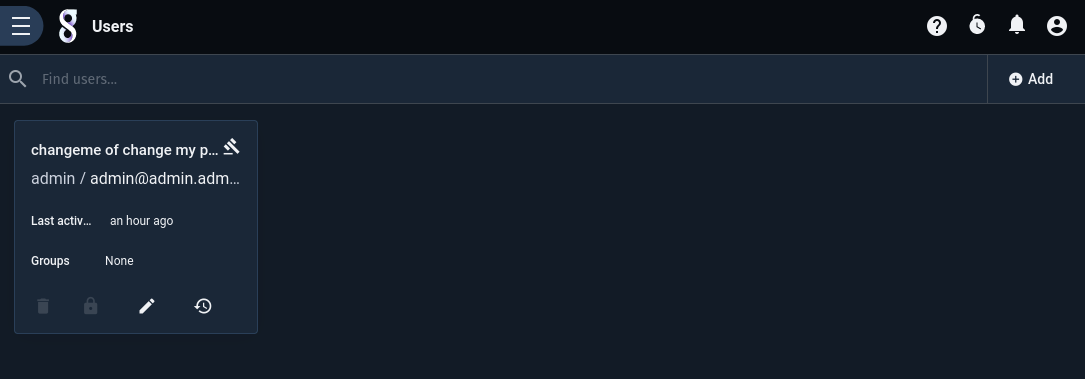
\includegraphics{images/users-admin.png}
	\caption{A Freshly-Installed System's User List}
	\label{fig:fresh-users}
\end{figure}

Clicking the `Add' button in the upper right brings up a dialog to
create a new user, as shown in Figure \ref{fig:newuser}. Note the 
`Administrator' checkbox at the bottom of the dialog. If this
box is checked, the user will receive administrator-level privileges.
Take care when selecting this option!


\begin{figure}
	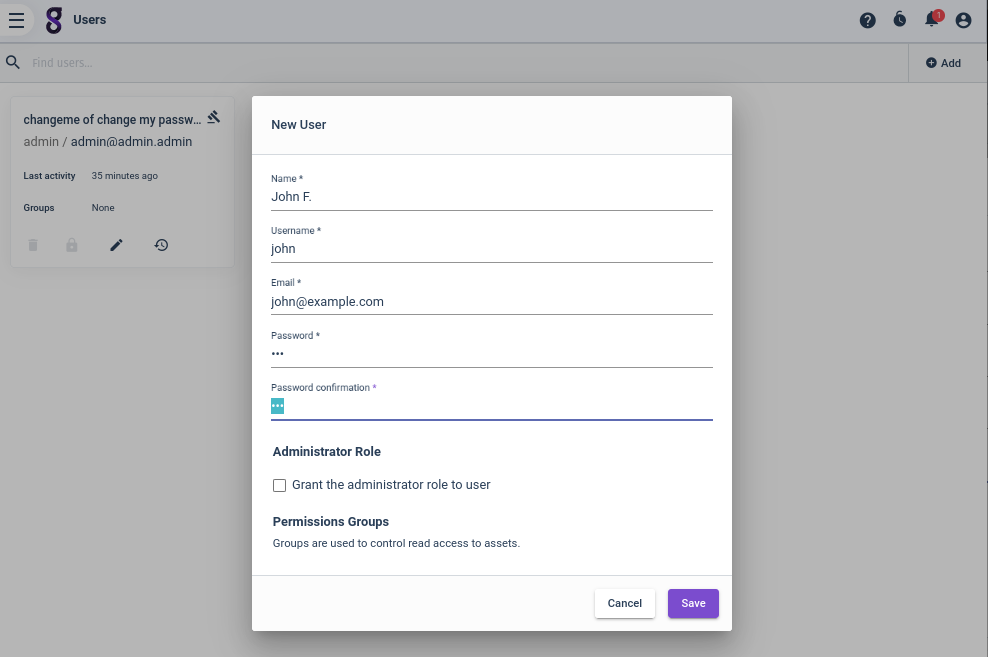
\includegraphics{images/newuser.png}
	\caption{New User Dialog}
	\label{fig:newuser}
\end{figure}


Each user information tile has four icons across the bottom, as shown in Figure \ref{fig:usertile}.
Selecting the trashcan icon will delete the user (prompting for
confirmation). The padlock icon will lock the user account, logging out
any sessions they may currently have and preventing them from logging in
again until the account is unlocked; this is a good way to deal with
misbehaving users. Both of these icons are disabled for the `admin'
user.

\begin{figure}
	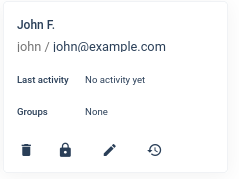
\includegraphics[width=0.5\linewidth]{images/usertile.png}
	\caption{The User Information Tile}
	\label{fig:usertile}
\end{figure}

The pencil icon brings up a dialog to edit the existing user, as shown in Figure \ref{fig:edituser}.
This allows you to reset the user's password, change their personal
information, or even make them an administrator if needed.

\begin{figure}
	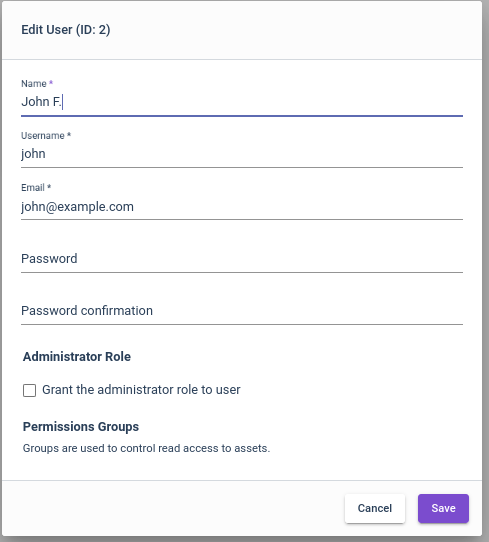
\includegraphics[width=0.55\linewidth]{images/edituser.png}
	\caption{Editing User Information}
	\label{fig:edituser}
\end{figure}

Finally, the clock icon brings up the user's search history, as shown in Figure \ref{fig:userhistory}.
This can be useful when attempting to help a user figure out why their searches
aren't working, or to keep an eye on what users are trying to extract
from your data.

\begin{figure}
	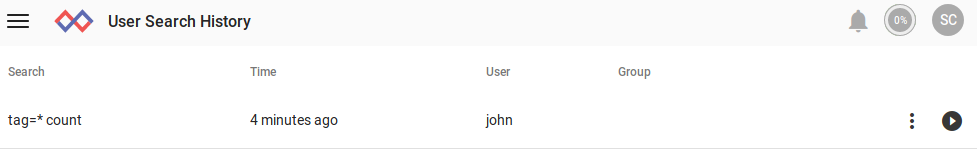
\includegraphics[width=0.9\linewidth]{images/userhistory.png}
	\caption{User Search History}
	\label{fig:userhistory}
\end{figure}

\section{Managing Groups}
\index{Groups}\index{GUI!groups}
Group management is very similar to user management. The Groups page in
the Administration section of the menu will initially show no groups, as in
Figure \ref{fig:fresh-groups}

\begin{figure}[H]
	
\includegraphics{images/empty-groups.png}
	\caption{A Freshly-Installed System's Group List}
	\label{fig:fresh-groups}
\end{figure}

A group can be added by clicking the `Add' button and filling out the
form, optionally selecting any users which should be members of the new
group, as shown in Figure \ref{fig:newgroup}

\begin{figure}
	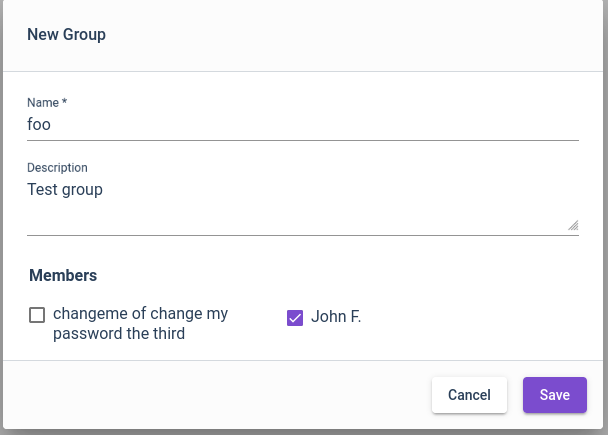
\includegraphics[width=0.6\linewidth]{images/newgroup.png}
	\caption{New Group Dialog}
	\label{fig:newgroup}
\end{figure}

Once created, a group's tile has three action icons as seen in Figure \ref{fig:grouptile}.
The trashcan icon deletes the group. The pencil icon allows the group
to be renamed or for members to be added/deleted. The clock icon shows
the history of searches which have been run which were accessible to
this group.

\begin{figure}
	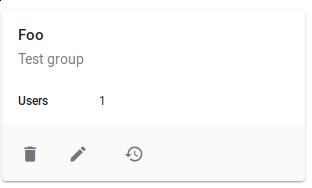
\includegraphics[width=0.5\linewidth]{images/grouptile.png}
	\caption{The Group Information Tile}
	\label{fig:grouptile}
\end{figure}

\clearpage
\section{Hands-on Lab: Managing Users and Groups}

First, launch a Gravwell webserver+indexer container:

\begin{Verbatim}[breaklines=true]
docker run --rm --net gravnet -p 8080:80 -d --name gravwell gravwell:base
\end{Verbatim}

Log into the web GUI (\href{http://localhost:8080}{http://localhost:8080}) and try the following tasks using the GUI:

\begin{enumerate}
\item
  Create a new user for yourself.
\item
  Create a new group and add your user to the group.
\item
  Log in as your user in a separate incognito window. From the admin
  account, lock your user account. What happened?
\end{enumerate}

To clean up after the experiment, run:

\code{docker kill \$(docker ps -a -q)}
